\documentclass[12pt]{article}


\usepackage{arxiv}

\usepackage[utf8]{inputenc} % allow utf-8 input
\usepackage[T1]{fontenc}    % use 8-bit T1 fonts
\usepackage{hyperref}       % hyperlinks
\usepackage{url}            % simple URL typesetting
\usepackage{booktabs}       % professional-quality tables
\usepackage{amsfonts}       % blackboard math symbols
\usepackage{amsmath}
\usepackage{nicefrac}       % compact symbols for 1/2, etc.
\usepackage{microtype}      % microtypography
\usepackage{lipsum}
\usepackage{graphicx}
\usepackage{caption}
\usepackage[gen]{eurosym} % euro sign

\usepackage{graphicx} % "demo" option just for this example
\usepackage{subcaption}
\usepackage{float}

\renewcommand{\baselinestretch}{1.5} 

%% BIB STUFF:
\usepackage[backend=bibtex,style=authoryear,natbib=true]{biblatex} % Use the bibtex backend with the authoryear citation style (which resembles APA)
\addbibresource{apt_bib.bib} % The filename of the bibliography
\usepackage[autostyle=true]{csquotes} % Required to generate language-dependent quotes in the bibliography
%\emergencystretch=1em % allows for an additional line-breaking pass with the amount of "tolerable" white space per line increased by 1em. Solving: Overfull hbox in biblatex (check StackExchange)
\setlength\bibitemsep{1.15\itemsep} % sep between bib entries in bibliography

\title{Mock Thesis: Regime Switching \\ {\large Combining Hierarchical Clustering-Based Asset Allocation \\ and News Sentiment}}


\author{
  Santiago~Walliser\\
  Department of B \& F\\
  University of Zurich\\
  Zurich\\
  \texttt{santiago.walliser@uzh.ch} \\
  %% examples of more authors
   \And
  Patrick~Lucescu \\
  Department of QF\\
  University of Zurich\\
  Zurich \\
  \texttt{patrick.lucescu@uzh.ch} \\
   \And
  Bjoern~Bloch \\
  Department of B \& F\\
  University of Zurich\\
  Zurich \\
  \texttt{bjoern.bloch@uzh.ch} \\
  %% \AND
  %% Coauthor \\
  %% Affiliation \\
  %% Address \\
  %% \texttt{email} \\
  %% \And
  %% Coauthor \\
  %% Affiliation \\
  %% Address \\
  %% \texttt{email} \\
  %% \And
  %% Coauthor \\
  %% Affiliation \\
  %% Address \\
  %% \texttt{email} \\
}

\begin{document}
\maketitle

\begin{abstract}
We present a new model independent approach based on the ideas of \citeauthor{enhPortOpti} who proved that news sentiment can be used in the context of SAA. We first construct portfolios based on a hierarchical clustering-based asset allocation approach and then we further adjust the portfolios' exposure to risky assets by using macro news sentiment data. Results are promising with geometric Sharpe Ratio between 0.6 and 0.86 for the portfolios with no News Sentiment enhancement. However, we are unable to draw any conclusions on the effectiveness of the News Sentiment enhancement. Nevertheless, we can identify the portfolio based on the "ward" method as the overall best performer among no News Sentiment enhanced portfolios while the portfolio based on the "single" method is the best performer among the News Sentiment enhanced portfolios.
\end{abstract}


% keywords can be removed
\keywords{ Strategic Asset Allocation, Regime Switching, News Sentiment, Hierarchical clustering-based asset allocation  }

%{\bfseries \emph Wordcount} \hspace{0.05cm} 2200



%%%%%%%%%%%%%%%%%%%%%%%%%%%%%%%%

\newpage
\section{Introduction}

Financial times series exhibit sudden breaks which lead to processes with completely other characteristics. Early identification of such regime switches (RS) are of major importance for strategic asset allocation (SAA). 

We propose a completely model independent approach for SAA in the context of RS, thereby allowing the data to speak for itself. In a first step, using a broad pool of different asset classes, we focus on a  hierarchical clustering-based asset allocation (HCBAA) which ensures us an 'all-weather' portfolio based on historical correlations. In a second step, we use the long lasting predictive power of news sentiment to decide if we are currently entering a bull or bear market cycle. Based on this insight we decide then if we should overweight bonds or equities for the next holding period. 

Our work is an extension of the research done by \citet{enhPortOpti} who focused on enhancing the traditional \citet{black1992global} SAA models with a behavioral based approach based on news sentiment. We circumvent the usage of a model by relying on the HCBAA approach which was first introduced by \citet{raffinot2017hierarchical} thereby extending the initial work of \citet{de2016building}. Applying classical and more novel hierarchical clustering methods to a selection of different asset classes, \citet{raffinot2017hierarchical} achieved truly diversified portfolios and achieved statistically better risk-adjusted performances. 

A short-coming of HCBAA, compared to the BL model, is the inability to introduce a forward looking estimate into the clustering procedure. However, we believe that our crude model independent procedure of over weighting specific asset classes depending on the differentiation between two cycles (bear or bull), is a more robust procedure. First, we are not required to create portfolios in order to induce our views into the weight generation procedure. Second, we circumvent all the common pitfalls of the classical mean-variance optimization procedure. 

Our results show that portfolios based on hierarchical clustering-based asset allocation methods are indeed efficient and are able to circumvent huge losses during times of high financial stress. Nevertheless, we are unable to improve our results by adjusting our risk exposure in times of high risks, which are predicted using macro news sentiment data.

The paper is structured as follows. In a first step, we position ourselves in the academic literature. We then discuss the methodology and the data with greater detail, followed by a presentation of the results. A final conclusion summarizes then main findings. 







%The academic literature has focused on identifying and predicting such changes in returns. Most of these regime switching (RS) models only allow for linear predictability, while others allow for non-linear regime dependent approaches (see for example \cite{ang2004regimes}).


\newpage
\section{State of the Art}

\subsection{Regime Switching}

There is clear evidence that not only expected returns but also volatility vary over time. Furthermore, it has been documented by \citet{longin1999correlation} that equity returns are highly correlated in times of high volatility, and that this relation is statistically significant. \citet{Ang2002InternationalAA} find that there are actually two regimes in the international equity market, and that these regimes exhibit the characteristics described by \citet{longin1999correlation}. As such, it is desirable from the strategic asset manager to adjust its exposure to asset classes according to the current market scenario. 

This has been coined in the literature as Regime Switching models. In the simplest form, regime switching (RS) models allows data to be drawn from two or more distributions which can be considered as our regimes. As such, at each point in time there is a probability that the process will be drawn from the same distribution or it will switch to another one. Of major importance is the work of \citet{hamilton1989new} which uses a Markov process to model the interplay of the different regimes.

\citet{ang2004regimes} further develop regime switching strategies and show that a global manager can add value by considering two scenarios, a bear or a bull market. However, it has been showed that frequent rebalancing can eat up the potential excess return of such strategies \citep{bauer2004timing}. Consequently, their practical application is limited.
\subsection{News Sentiment}

In the past decade the literature on News Sentiment Analysis has advanced tremendously due to the technological improvements in evaluation of large data sets. This has been a direct result of the improvements of Natural Language Processing algorithms as well as the evolution of computational power of computers. On the other hand, news sentiment has become a core part of behavioural finance. Among the first papers that discuss this topic is \cite{tetlock2007giving}, who found a correlation between negative news and negative future equity returns. Since then the predictive power has been shown to be persistent for weeks and months (\citet{uhl2015s}) rather than days as it was shown by \citet{tetlock2007giving}.

While most of the academic papers on news sentiment focus on investment time horizons of days, weeks or months, \citet{enhPortOpti} attempt to use long-term news sentiment in an SAA framework. They use long-term news sentiment momentum, as constructed by \citeauthor{uhl2015s}, in a Black-Litterman (BL) framework together with the classical mean variance optimization in order to derive the optimal weights deviation from a predefined benchmark. \citeauthor{enhPortOpti} are thus able to enhance the Sharpe Ratios of the benchmark SAAs by almost $20\%$. Nevertheless, the use of BL and  mean variance optimization comes with its own drawbacks. Besides the dimensionality curse of both BL and mean variance, in the BL framework the portfolio manager must form linear views on the assets which are assumed to be uncorrelated. However, in practice views correlations might exist but can be hard to quantify. 







 
\subsection{Hierarchical Clustering-Based Asset Allocation}

Since its inception in 1952, Markowitz's theory has been proven to be a significant stepping stone in modern portfolio construction. Despite its advertised diversification benefits, Markowitz's optimal portfolio exhibits some complications which make it somewhat unreliable in practice. 

It is worth mentioning here the conditioning number of a matrix, which is the absolute value of the ratio between its maximal and minimal eigenvalues. The more correlated the investments, the higher the conditioning number which leads to unstable matrix inversion as a small change in one of the entries of the covariance matrix can lead to a completely different inverse. Consequently, Markowitz's curse states that the more correlated the investments, the greater the need for diversification, and yet the more likely we will receive unstable solutions. This is due to estimation erros in the covariance matrix.

\citet{de2016building} introduces a portfolio diversification technique called "Hierarchical Risk Parity" (HRP) to address three major concerns with Markowitz's approach: instability, concentration and underperformance. It uses graph theory and machine learning techniques and one of the main advantages over quadratic optimizers is that it can compute a portfolio on an ill-degenerated or even a singular covariance matrix. The starting point of his analysis is that the correlation matrix lacks a hierarchical structure and as such it cannot differentiate between assets. As \citet{raffinot2017hierarchical} states: "Hierarchical clustering refers to the formation of a recursive clustering, suggested by the data, not defined a priori. The objective is to build a binary tree of the data that successively merges similar groups of points." \citet{de2016building} shows that this approach delivers lower out-of-sample variance than CLA or traditional risk parity methods (IVP).


\citet{raffinot2017hierarchical} extends this idea by considering several variants of hierarchical clustering algorithm (Simple Linkage, Complete Linkage, Average Linkage, Ward’s Method). He concludes that the resulting portfolios are indeed diversified and achieve higher Adjusted Sharpe Ratios compared to standard methods.





\newpage
\section{Methodology}

\subsection{Asset Allocation}

In a first step, we focus on the computation of the HCBAA weights. Let $f$ represent the HCBAA algorithm, which at time $t$ takes as input the asset correlation matrix $\mathbf{\Sigma_t^T}$ with a lookback window of $T$ periods as well as the desired clustering \texttt{method}. We make use of all the different presented clustering algorithms in order to compare their performances and therefore \texttt{method} $\in$ \{\texttt{single, complete, average, ward}\}. The function $f$ outputs then the corresponding robust weight vector $\mathbf{w_t^{HCBAA}}$ which contains the for each asset $i$ the corresponding weight $w_{t,i}^{HCBAA}$:
\begin{align}
    f(\mathbf{\Sigma_t^T}, \text{\texttt{method}}) = \mathbf{w_t^{HCBAA}}
\end{align}

The length of the lookback window $T$ is a hyper-parameter which can be tuned via cross validation. 

In a second step, we focus on adjusting the risk of our exposure based on our prediction which relies on news sentiment. Latter time series ranges from $-1$ to $+1$, where a negative value indicates a negative sentiment and vice-versa. For this we create three groups of sub-asset classes: 

\begin{itemize}
    \item \textbf{High risk assets} which include equities
    \item \textbf{Low risk assets} which include bonds
    \item Non-risk-categorized assets such as infrastructure indices
\end{itemize}{}

In order to overweight our exposure to a sub-asset class at time $t$ we proceed as follows. Let $\lambda > 1$ be the factor by which the exposure is  increased. Further, let $j$ $\in$ \{\texttt{high risk, low risk}\} such that $o_{j,i}$ equals $\lambda$ if asset $i$ belongs to the sub-asset class indexed by $j$, otherwise $1$. Then, $\mathbf{o_j}$ is a vector which contains these $o_{j,i}$ values.  To adjust our allocation we modify $\mathbf{w_t^{HCBAA}}$ using $\mathbf{o_j}$ thereby obtaining our regime adjusted weights $\mathbf{w_t^{RA'}}$. For $N$ assets we have therefore following (exemplary) relation:

\begin{equation}
    \mathbf{w_t^{RA'}} = \mathbf{w_t^{HCBAA}} * \mathbf{o_j} = \left( \begin{matrix} w_{t,1}  \\ \vdots  \\ w_{t,N} \\ \end{matrix} \right) * \left( \begin{matrix} \lambda  \\ \vdots  \\ 1 \\ \end{matrix} \right)
\end{equation}{}

In order to regain an exposure of 100\% we re-normalize $\mathbf{w_t^{RA'}}$ such that the total sum of vector's element equals one again, yielding us the final regime adjusted weight vector $\mathbf{w_t^{RA}}$.

\subsection{Investment Procedure}

This weight finding procedure is repeated at every rebalancing key date. In the spirit of SAA, we rebalance every 12 month. We hold the same exposure during the whole holding period. 

We initialize our research with a lookback window length $T$ of 12 months.  

The $\lambda$ parameter allows investors to induce their risk-tolerance into the investment procedure. In order to have clearly distinguishable results, we set this factor to $2$, i.e. we double our exposure to the regime appropriate sub-asset class.


\newpage
\section{Data}

\subsection{Assets}

Table \ref{available_assets} presents the different available asset classes and their corresponding classification into the different sub-asset classes. The selection and hedging of the asset classes assumes an investor based in Switzerland. The decision with respect to the categorization of the assets is solely based on the beta. 



\begin{table}[h!]
\centering
\begin{tabular}{@{}lcccc@{}}
\toprule
\textbf{Asset}                                    & \textbf{Low Risk} & \textbf{High Risk} & \textbf{Beta} & \textbf{Standard Deviation} \\ \midrule
Bonds CHF                                         & $X$               &              &  0.008    &  0.867   \\
Bonds Global Government (CHF hedged)              & $X$               &              &  -0.002    &  1.105   \\
Bonds Global (CHF hedged)                         & $X$               &              &   0.043   &  1.185   \\
Gold                                              & $X$               &              &  0.173    &  5.246   \\
Equities Switzerland                              &                   & $X$          &  0.692    &   4.641  \\
Equities Global Developed                          &                   & $X$          &  1.000    &   4.840  \\
Equities Emerging Markets                         &                   & $X$          &  1.100    &   6.447  \\
Equities Global Small Cap                         &                   & $X$          &  1.021    &   5.196  \\
Private Equity                                    &                   & $X$          &  1.070    &   5.936  \\
Bonds Emerging Markets hard currency (CHF hedged) &                   &              &  0.310   &   3.063  \\
Bonds Emerging Markets local                      &                   &              &  0.647    &  3.881   \\
Insurance-Linked Securities (desmoothed)          &                   &              &  0.379    &  3.230   \\
Infrastructure                                    &                   &              &  0.766    &   3.959  \\ \bottomrule
\end{tabular}
\caption{List of available assets and their categorization into the three different sub-asset classes. Betas and standard deviations computed from 31.01.1972 to 31.08.2019 using the MSCI Global as benchmark.}
\label{available_assets}
\end{table}

\subsection{News Sentiment}
We make use of the same data set used by \citet{uhl2015s}. The data is provided by Thomson Reuters, a leading provider of sentiment-classified news in the industry. 

As we are investing globally in the context of SAA and RS we focus on the macro news sentiment, which includes following macro-specific indicators \citep[p. 103]{uhl2015s}:

\begin{itemize}
    \item Monetary Policy/ Central Bank Actions
    \item Economic Indicators
    \item Credit/ Government Debt Ratings
    \item Politics/ War/ Environment
\end{itemize}

Using these indicators each news document is analyzed for its positive, neutral, and negative sentiment. A weight between 0 and 1 is then assigned to each sentiment, under the condition that the sum of the weights equals 1. The final sentiment weight that is assigned to a news document is the largest of those three sentiments. All these final news sentiment values are averaged for every day. We end up with a daily time series of macro-economical news sentiment.

As the daily observations are very noisy, we use a 10 day rolling exponential weighted mean in order to weight news sentiment in the near past slightly more. Next, we remove any forward looking bias by shifting data by one day forward. We aggregate the data then to monthly by summing monthly news sentiment values up. We believe, that the total news sentiment in a given month is a good proxy for the momentary overall market sentiment. We remark at this point, that results do not change if non-aggregated daily observations are used. In a final step, we normalize the complete data series such that the values lay in the range of -1 and 1. 

%Figure \ref{fig:news_sentiment} presents the final monthly time series.

% Die positive, neutral, negative werden jeweils pro Single News Artikel ausgewiesen wobei diese pro Artikel immer auf 100% summieren. Die avgSentimentClass wird dann gemäss dem höchsten Wert der drei (also pos, neg, neut) bestimmt. Ich nehme dann alle Werte pro Tag in der jeweiligen Kategorie und bilde einen gleichgewichteten Durchschnitt gemäss der Anzahl der News. Neutral sind Textpassagen, die entweder nicht zugewiesen werden können oder einfach weder positiv noch negativ ist.

% Exponential Weighted Moving Average to emphasize data in the near past. We compute the mean using windows of 360 days. 
% We remove any forward looking bias by shifting data by one day forward. 
% Resample to monthly by summing up the values
% Normalize data then to +1 and -1


% ---

% Thomson Reuters is one of the few providers of 

%\cite{uhl2015s}

% \begin{figure}[H]
%     \centering
%     \includegraphics[width=\linewidth]{Plots_and_Tables/news_sentiment.png}
%     \caption{News Sentiment}
%     \label{fig:news_sentiment}
% \end{figure}{}
\newpage
\section{Results}

%Two step appraoch of result presentation using two different approaches with different BMs
This section provides an overview of the results while in the next section we discuss them. 

Subfigure \ref{fig:notc_noNS_perf} provides an overview of all portfolios without News Sentiment enhancement and no transaction costs. Subfigure \ref{fig:tc_noNS_perf} provides the same overview but this time the solid line represents the performance without transaction costs while the dotted lines include transaction costs of 25 basis points. Furthermore, both subfigures \ref{fig:notc_noNS_perf} and \ref{fig:tc_noNS_perf} include our benchmarks: "BM Eq" which represents the equally weighted portfolio while "BM Ivp" represents the inverse volatility portfolio. Table \ref{stats} provides summary statistics of the four portfolios as well as for the two benchmarks.

Subfigure \ref{fig:notc_NS_perf} plot the portfolio performance when News Sentiment enhancement is added but with no transaction costs. In subfigure \ref{fig:tc_NS_perf} the dotted lines include transaction costs of 25 basis points. 


% STATISTICS TABLE
\begin{table}[h]
\centering
    \begin{tabular}{lcccccc}
                         & Single & Complete & Average & Ward  & BM Ivp & BM Eq  \\
    \midrule
    Geometric Average Excess Return      & 0.39   & 0.45     & 0.39    & 0.5   & 0.25   & 0.4   \\
Geometric Average Total Return   & 0.45   & 0.49     & 0.43    & 0.54  & 0.3    & 0.45  \\
Arithmetic Average Total Return & 0.46   & 0.49     & 0.44    & 0.54  & 0.29   & 0.46  \\
Arithmetic Average Excess Return    & 0.42   & 0.47     & 0.41    & 0.52  & 0.25   & 0.44  \\
Standard Deviation Excess Returns         & 2.27   & 2.01     & 2.0     & 2.0   & 0.85   & 2.45  \\
Sharpe Ratio Arithmetic     & 0.63   & 0.8      & 0.7     & 0.9   & 1.04   & 0.61  \\
Sharpe Ratio Geometric      & 0.6    & 0.77     & 0.67    & 0.86  & 1.02   & 0.57  \\
Minimum Excess Return          & -8.13  & -8.74    & -7.59   & -8.03 & -3.2   & -13.0 \\
Maximum Excess Return          & 7.87   & 7.73     & 7.92    & 7.15  & 3.13   & 8.23  \\
Skewness Excess Return         & -0.24  & -0.56    & -0.4    & -0.46 & -0.35  & -1.23 \\
Kurtosis Excess Return         & 2.17   & 2.84     & 2.31    & 2.16  & 1.35   & 5.0  \\
    \bottomrule
    \end{tabular}
    \\[5pt]
     \captionsetup{width=0.925\linewidth}
     \caption[Summary statistics of the four different portfolios together with the two benchmark for no News Sentiment enhancement.]{Summary statistics of the four different portfolios (Single, Complete, Average and Ward) together with the two benchmarks for no News Sentiment enhancement. Data is monthly with the Sharpe Ratios annualized.}
    \label{stats}
\end{table}


% PERFORMANCE NO NS ENHANCEMENT
\newpage
\begin{figure}[H] % "[t!]" placement specifier just for this example
\centering

\begin{subfigure}{0.8\textwidth}%{0.48\textwidth}
\centering
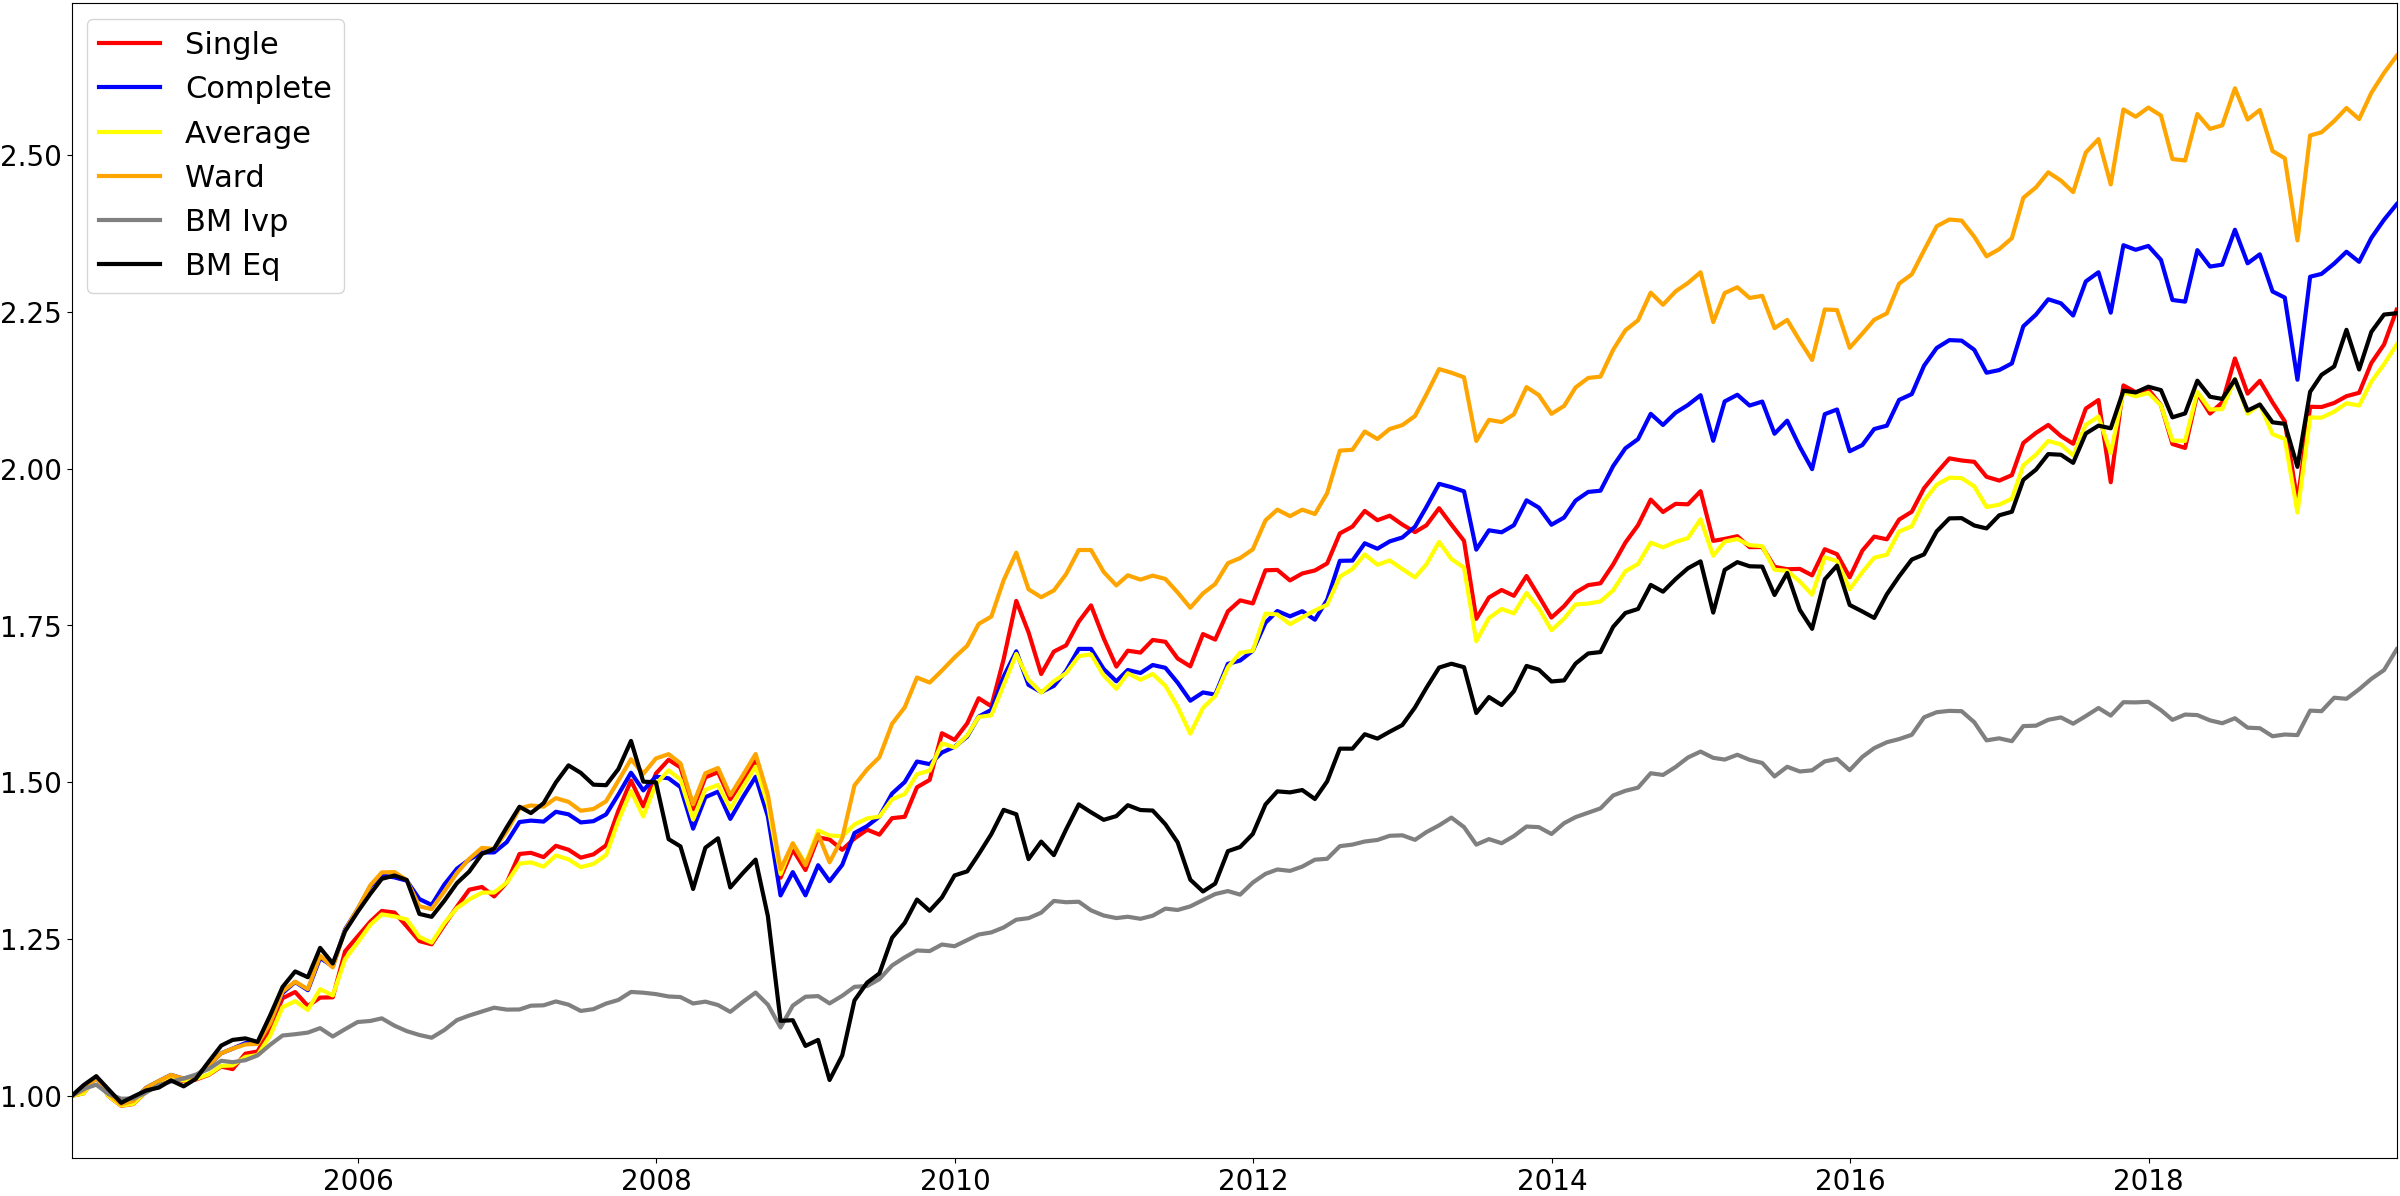
\includegraphics[width=\linewidth]{Plots_and_Tables/perf_noTC_without_NS_F_1_B_0_LB_12_0.png}
\caption{Performance of strategies excluding transaction costs.} \label{fig:notc_noNS_perf}
\end{subfigure}%\hspace*{\fill}

\medskip
\begin{subfigure}{0.8\textwidth}%{0.48\textwidth}
\centering
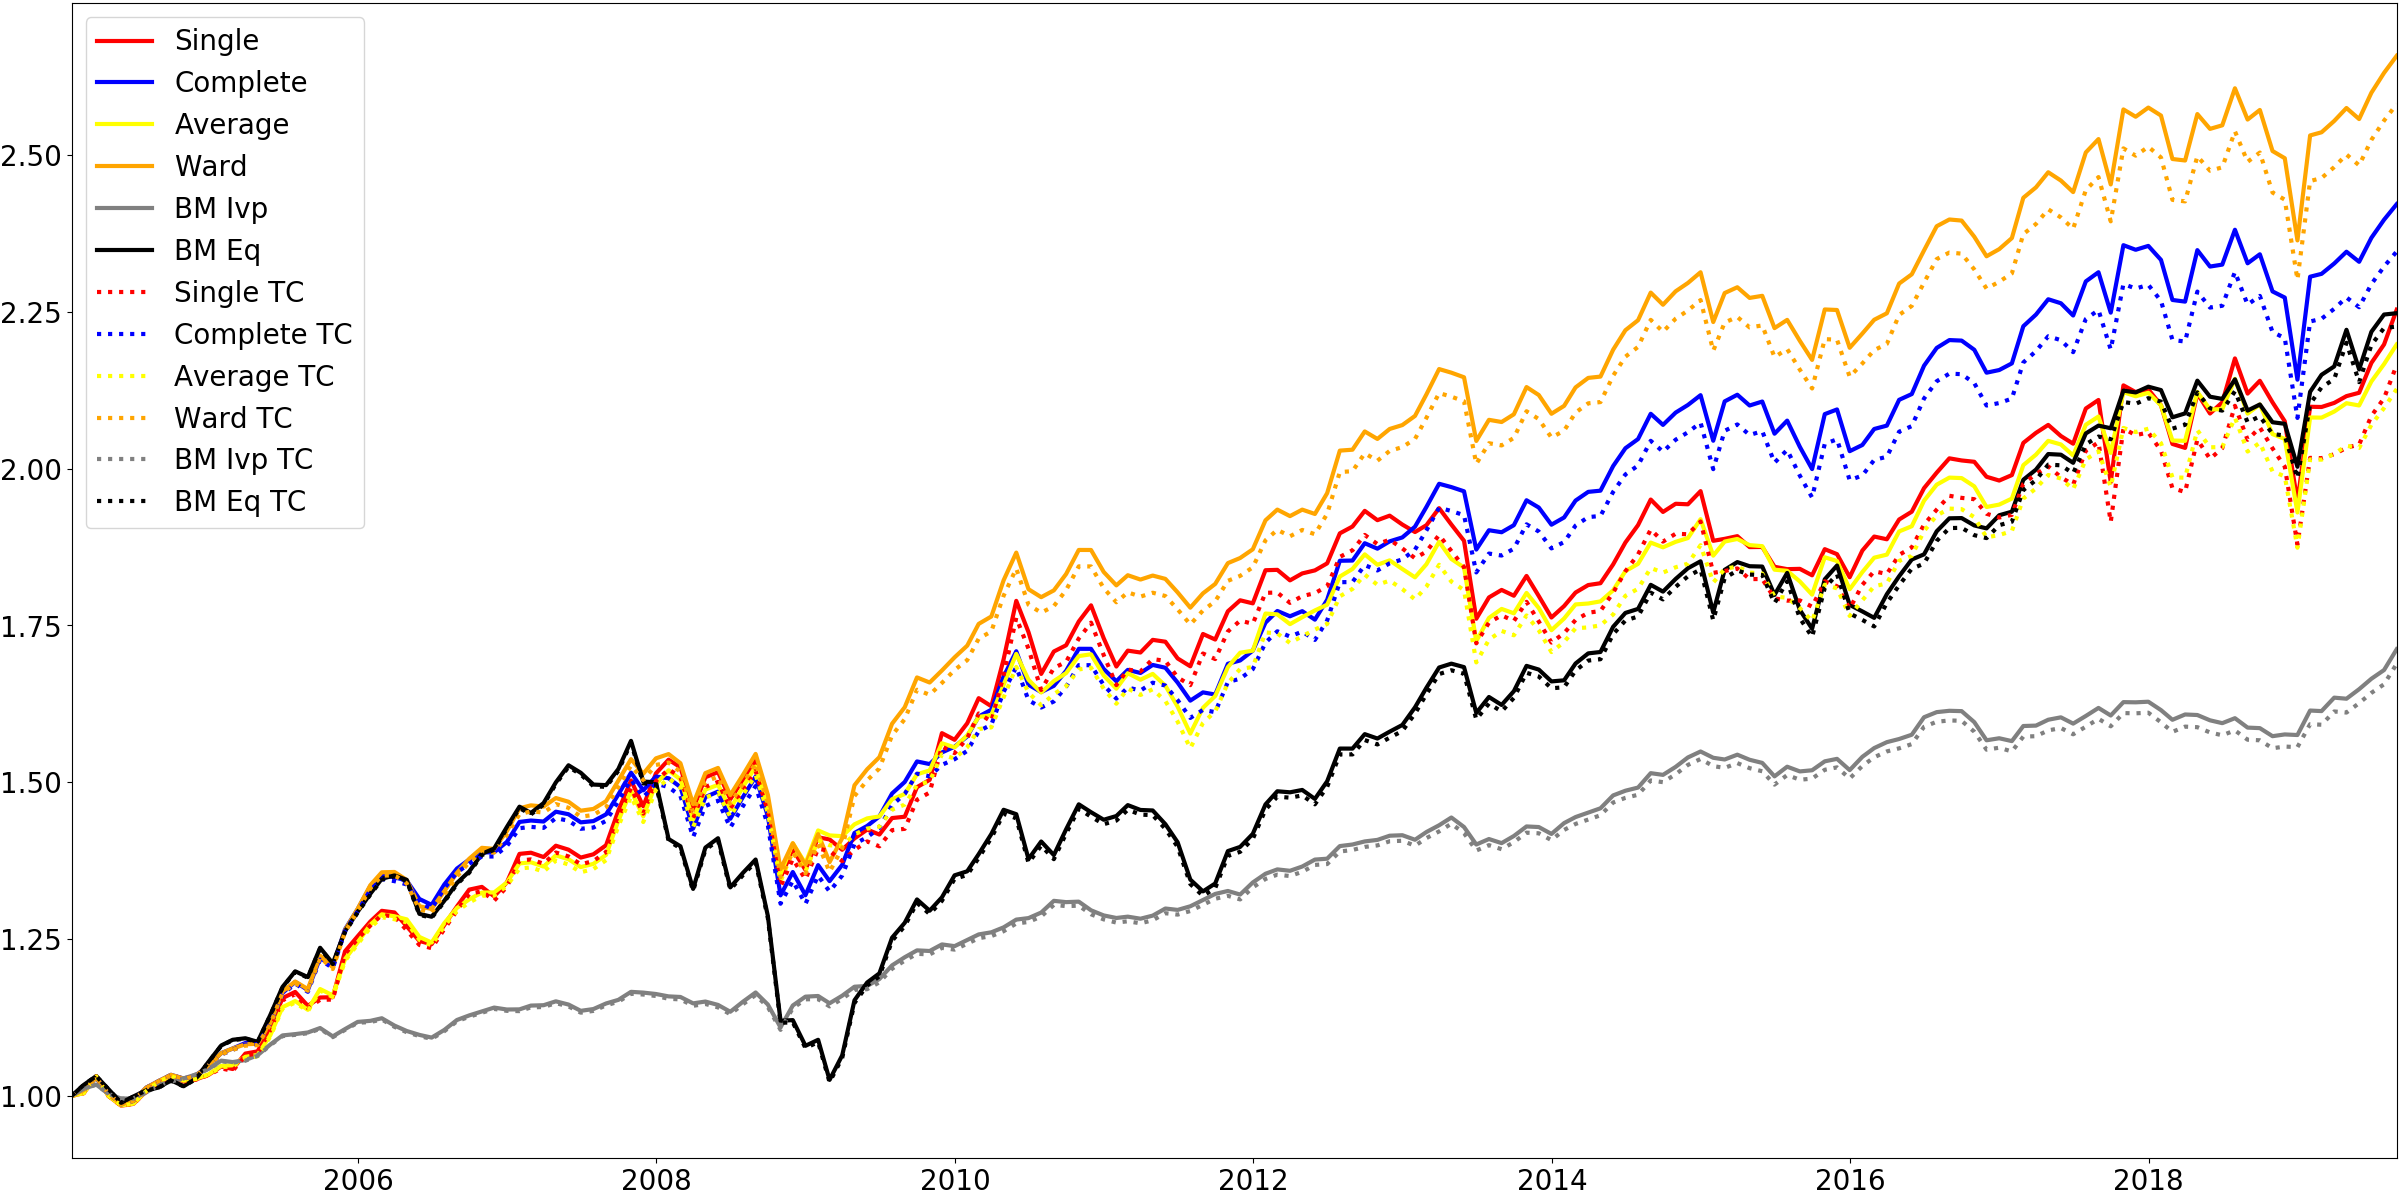
\includegraphics[width=\linewidth]{Plots_and_Tables/perf_noTC_andTC_without_NS_F_1_B_0_LB_12_0.png}
\caption{Performance of strategies including transaction costs.} \label{fig:tc_noNS_perf}
\end{subfigure}%\hspace*{\fill}


% \medskip
% \begin{subfigure}{0.8\textwidth}%{0.48\textwidth}
% \centering
% \includegraphics[width=\linewidth]{Plots_and_Tables/AA_without_NS_F_1_B_0_LB_12_0.png}
% \caption{Comparison of strategy performances with and without transaction costs.} \label{fig:comp_noNS_perf}
% \end{subfigure}%\hspace*{\fill}


\caption{Performance of different strategies without News Sentiment enhancement.} \label{fig:noNS_perf}
\end{figure}
\newpage
\newpage
\begin{figure}[H] % "[t!]" placement specifier just for this example
\centering

\begin{subfigure}{0.8\textwidth}%{0.48\textwidth}
\centering
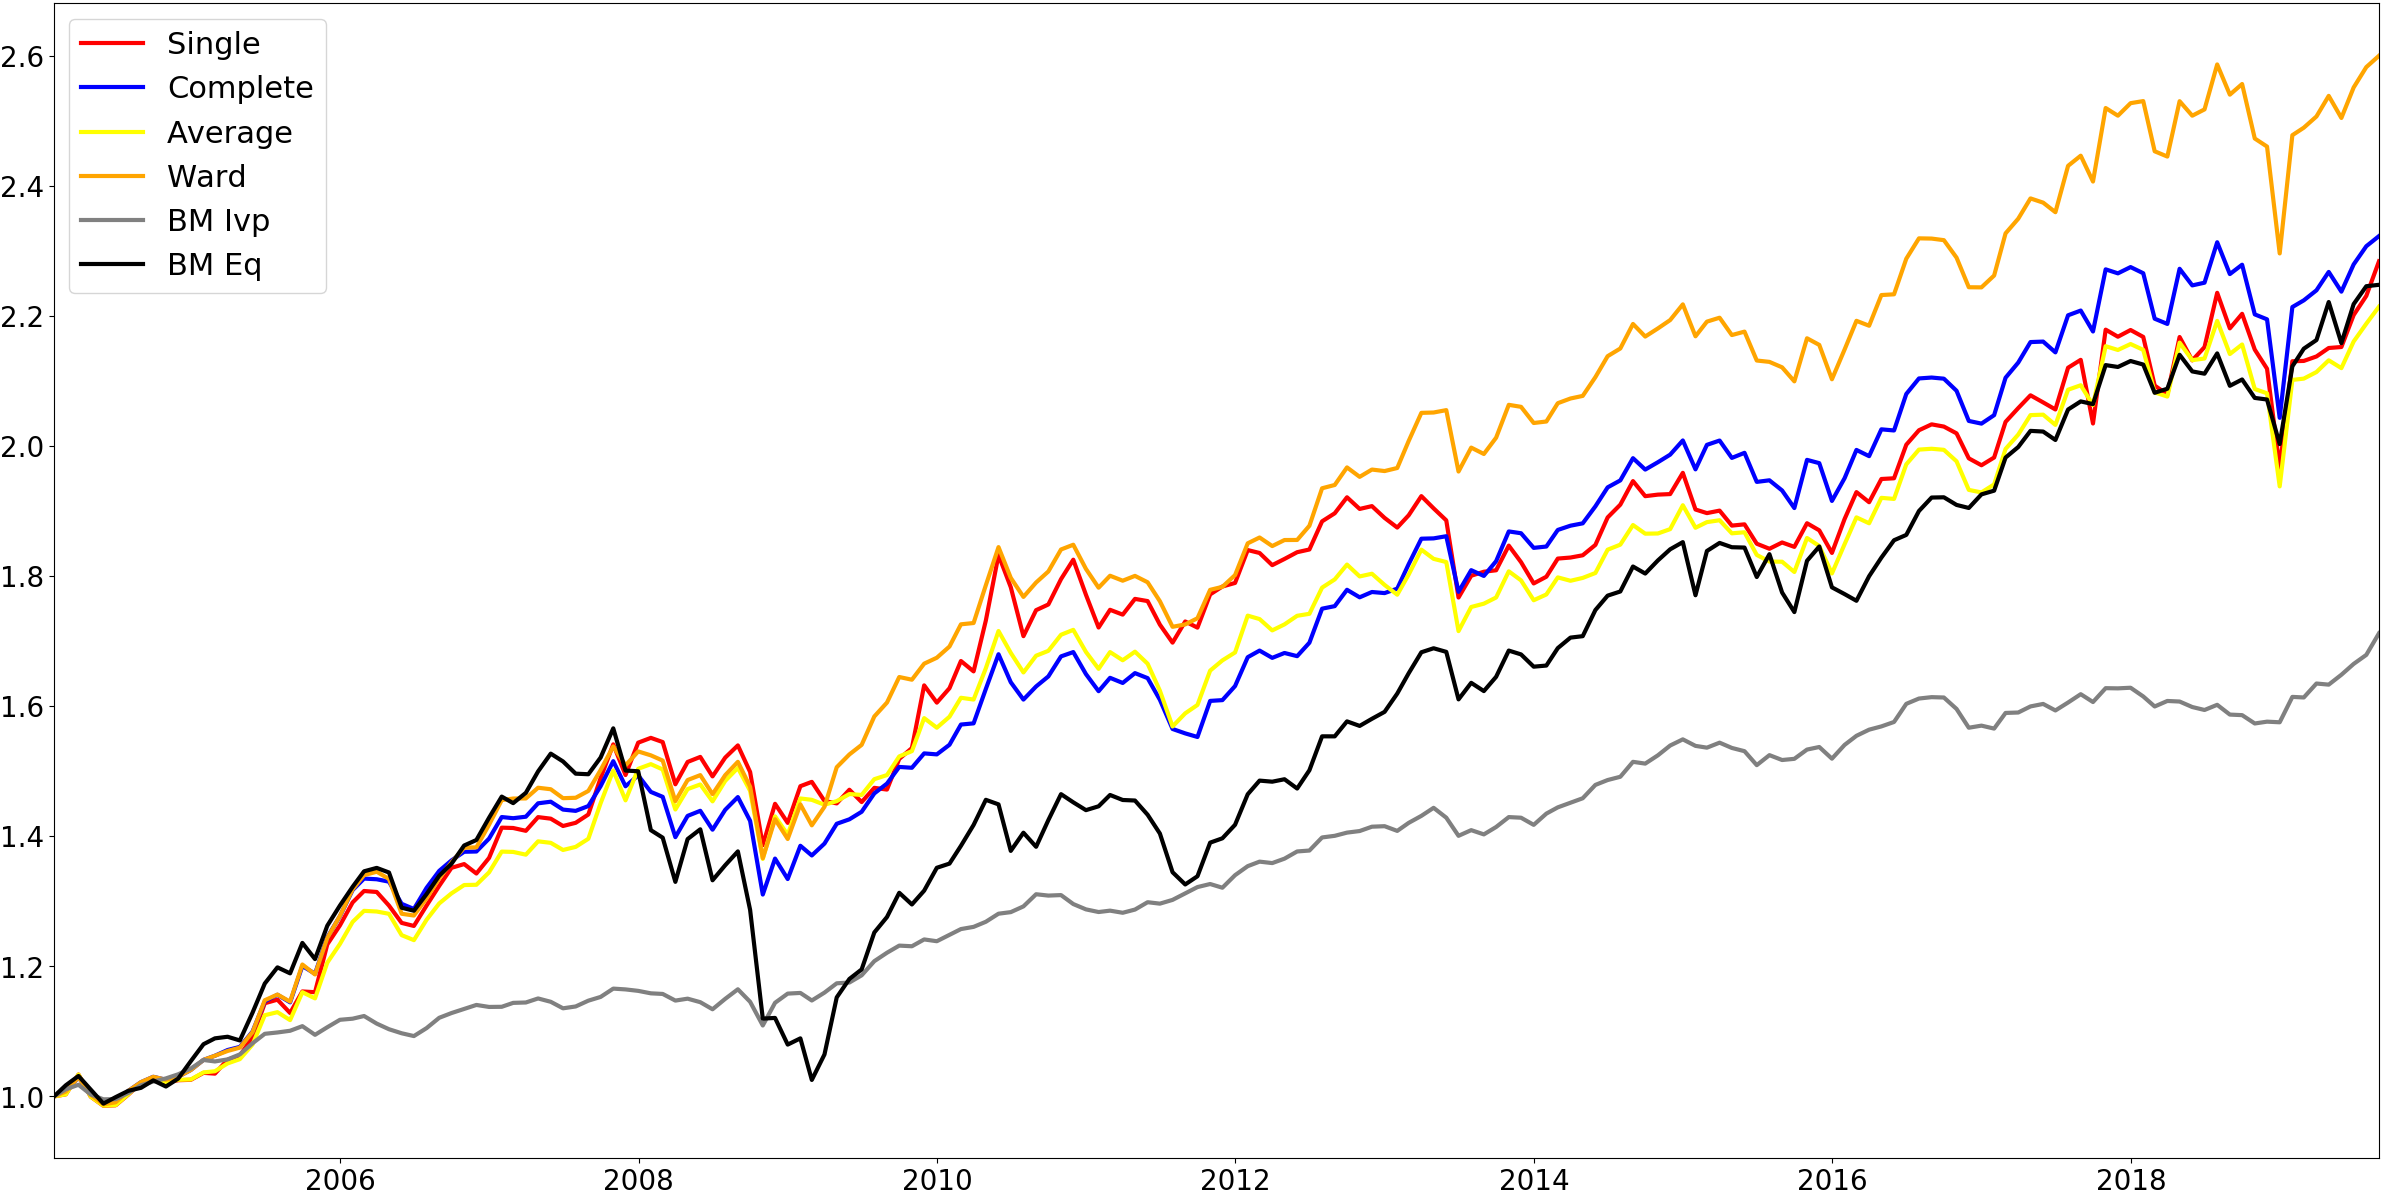
\includegraphics[width=\linewidth]{Plots_and_Tables/perf_noTC_with_NS_F_2_B_0_LB_12_0.png}
\caption{Performance of strategies excluding transaction costs.} \label{fig:notc_NS_perf}
\end{subfigure}%\hspace*{\fill}

\medskip
\begin{subfigure}{0.8\textwidth}%{0.48\textwidth}
\centering
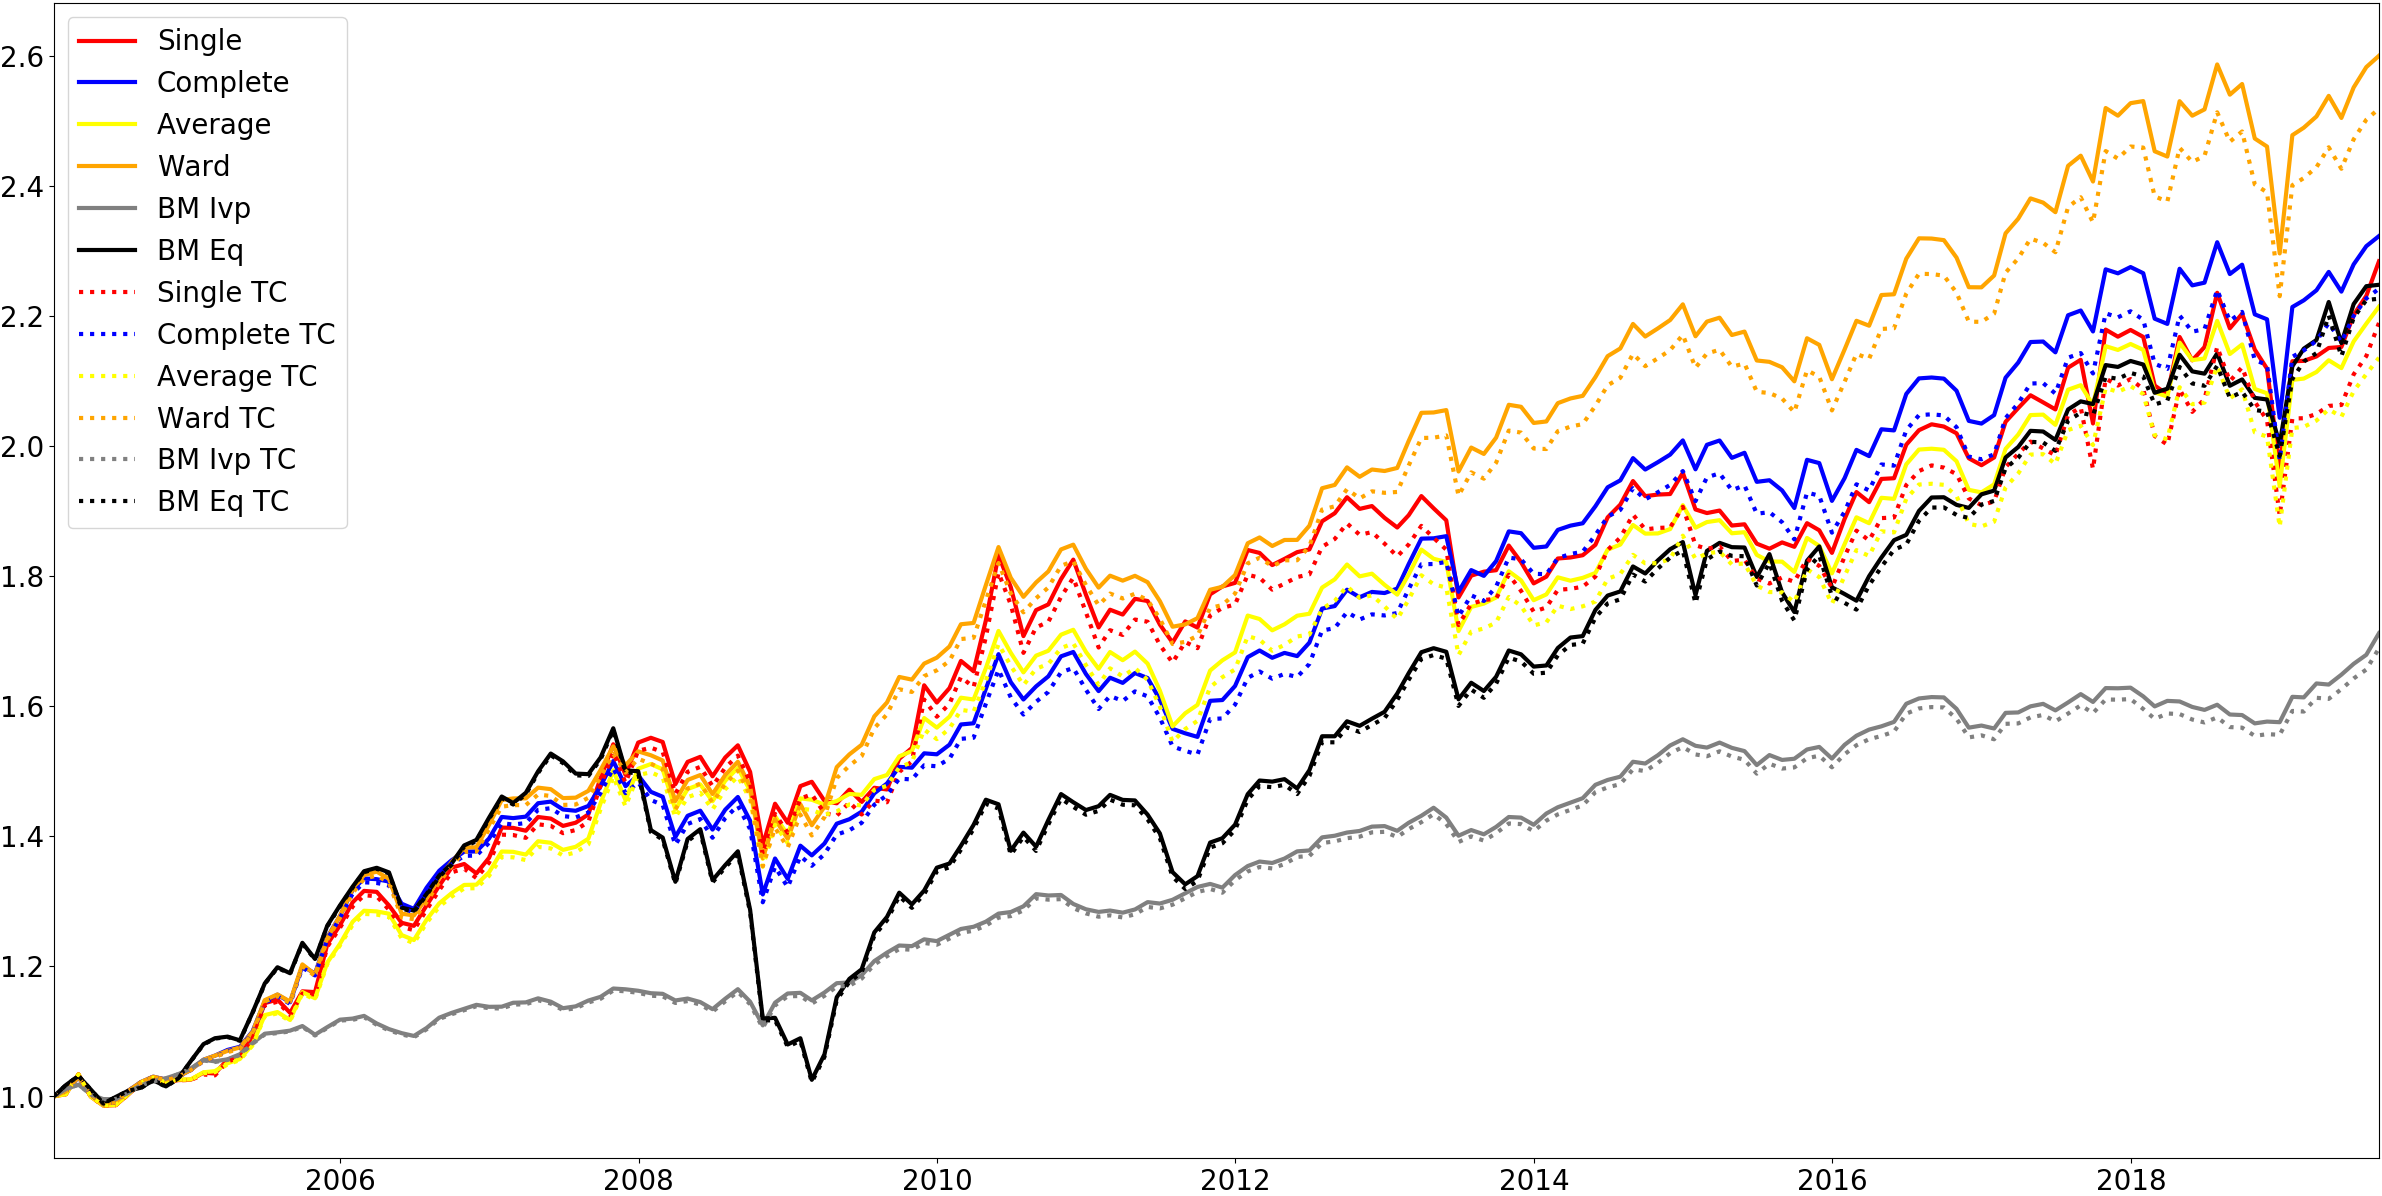
\includegraphics[width=\linewidth]{Plots_and_Tables/perf_noTC_andTC_with_NS_F_2_B_0_LB_12_0.png}
\caption{Performance of strategies including transaction costs.} \label{fig:tc_NS_perf}
\end{subfigure}%\hspace*{\fill}


% \medskip
% \begin{subfigure}{0.8\textwidth}%{0.48\textwidth}
% \centering
% \includegraphics[width=\linewidth]{Plots_and_Tables/AA_with_NS_F_2_B_0_LB_12_0.png}
% \caption{Comparison of strategy performances with and without transaction costs.} \label{fig:comp_NS_perf}
% \end{subfigure}%\hspace*{\fill}


\caption{Performance of different strategies with News Sentiment enhancement.} \label{fig:noNS_perf}
\end{figure}
\newpage
%\newpage
\begin{center}

\begin{figure}[H] % "[t!]" placement specifier just for this example
\centering
\begin{subfigure}{1\textwidth}%{0.48\textwidth}
\centering

\includegraphics[width=\linewidth]{Plots_and_Tables/AA_step1_F_1_B_0_LB_12.png}
\caption{Allocation without News Sentiment enhancement.} \label{fig:notc_NS_perf}
\end{subfigure}%\hspace*{\fill}

\medskip
\begin{subfigure}{1\textwidth}%{0.48\textwidth}
\centering
\includegraphics[width=\linewidth]{Plots_and_Tables/AA_step1_F_2_B_0_LB_12.png}
\caption{Allocation with News Sentiment enhancement.} \label{fig:tc_NS_perf}
\end{subfigure}%\hspace*{\fill}

\caption{Comparison of allocations of strategies with an without NS enhancement.} \label{fig:noNS_perf}
\end{figure}

\end{center}
\newpage





\newpage
\section{Discussion}

When looking at Figure \ref{fig:noNS_perf} we observe that all portfolio considered perform better than the inverse volatility benchmark as well as the equally weighted benchmark. Specifically, the portfolios return monthly geometric average total return between 0.43\% and 0.54\% while the the benchmarks achieve 0.3\% in the case of the inverse volatility benchmark and 0.45\% in the case of the equally weighted benchmark. In terms of Geometric Sharpe Ratio the portfolio using the "ward" method is by far the most appealing one, with 0.86, although it falls short of the inverse volatility benchmark which achieves a Geometric Sharpe Ratio of 1.02 due to its far lower standard deviation. It is of particular interest to notice that all four portfolios exhibit negative skewness and kurtosis below 3. Furthermore, we observe the same pattern when we consider the News Sentiment enhanced portfolios.

As the portfolio based on the "ward" method is the clear winner between the four portfolios consider, we focus our attention now to the comparison of the portfolio with and without News Sentiment. Following the approach of \citet{enhPortOpti} we run our benchmark for different starting month in order to check for robustness. The result is displayed in Figure \ref{fig:noNS_perf}. Unfortunately we cannot draw a conclusion on the effectiveness of the News Sentiment enhancement as there is no clear winner between the two approaches. 

Motivated by the fact that even the magnitude of the performance of the two portfolios varies across the chosen starting month of the portfolio we run 12 backtest, one for each month of the year. This robustness check is done for both with or without News Sentiment enhancement. Results are displayed in Appendix 1. It can be observed that the portfolios are not robust and that their performance varies with the month selected. However, it can be seen that overall "ward" performs the best when there is no News Sentiment enhancement while "single" performs the best among the News Sentiment enhanced portfolios.


\newpage
\begin{figure}[H] % "[t!]" placement specifier just for this example
\centering

\begin{subfigure}{0.8\textwidth}%{0.48\textwidth}
\centering
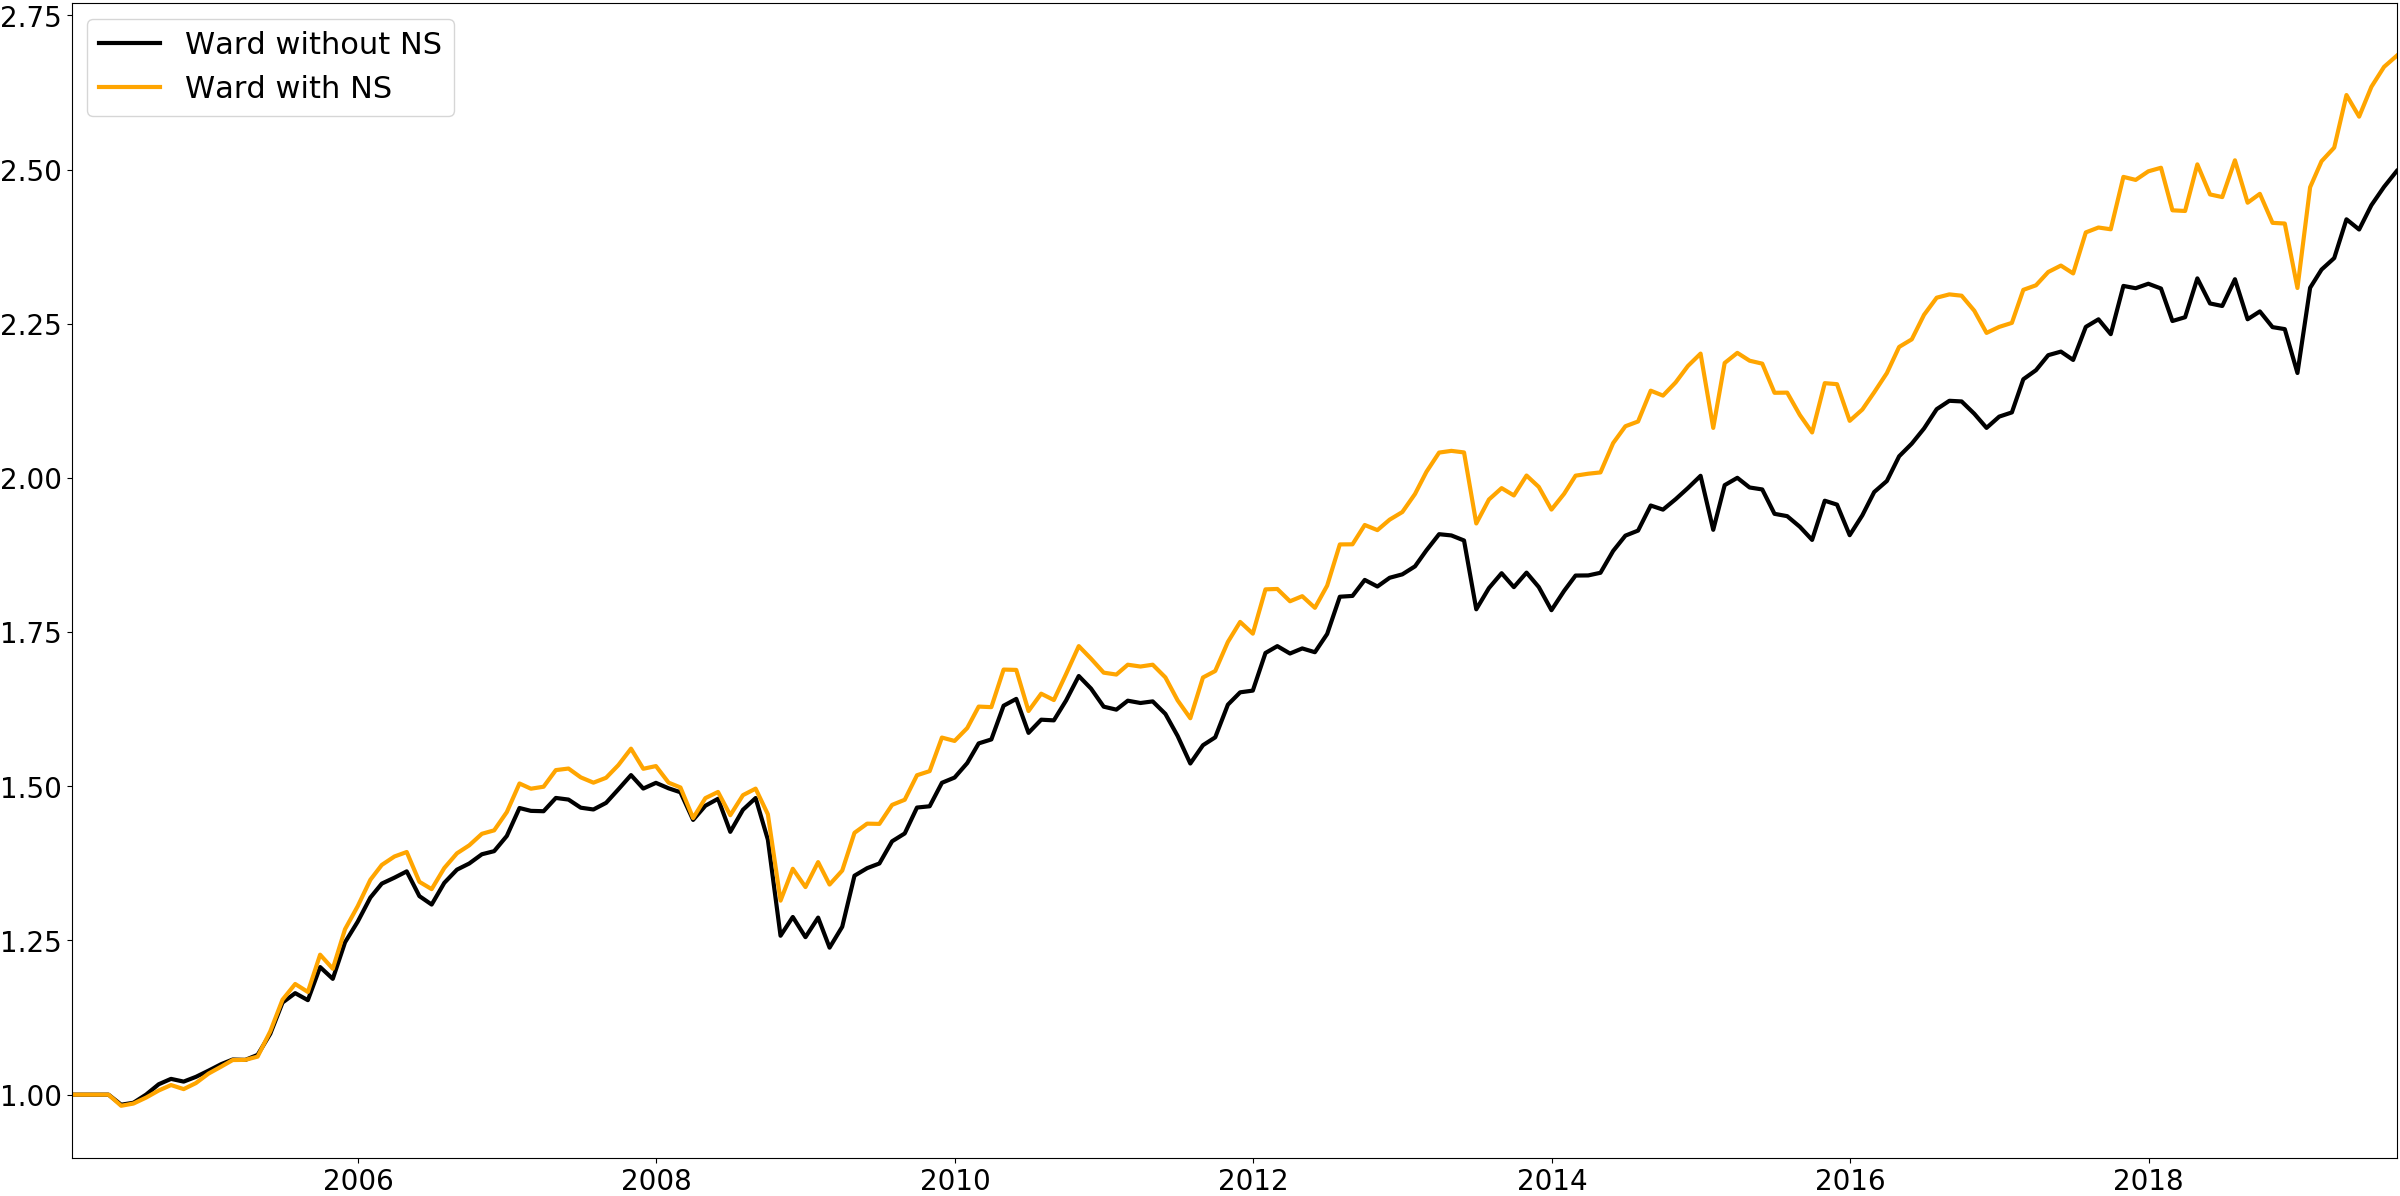
\includegraphics[width=\linewidth]{Plots_and_Tables/perf_noTC_ward_comp_F_2_B_0_LB_12_3_!!}
\caption{Comparison \texttt{ward} clustering approach with and without News Sentiment starting in May 2004.} \label{fig:notc_noNS_perf} % 3 + 2
\end{subfigure}%\hspace*{\fill}

\medskip
\begin{subfigure}{0.8\textwidth}%{0.48\textwidth}
\centering
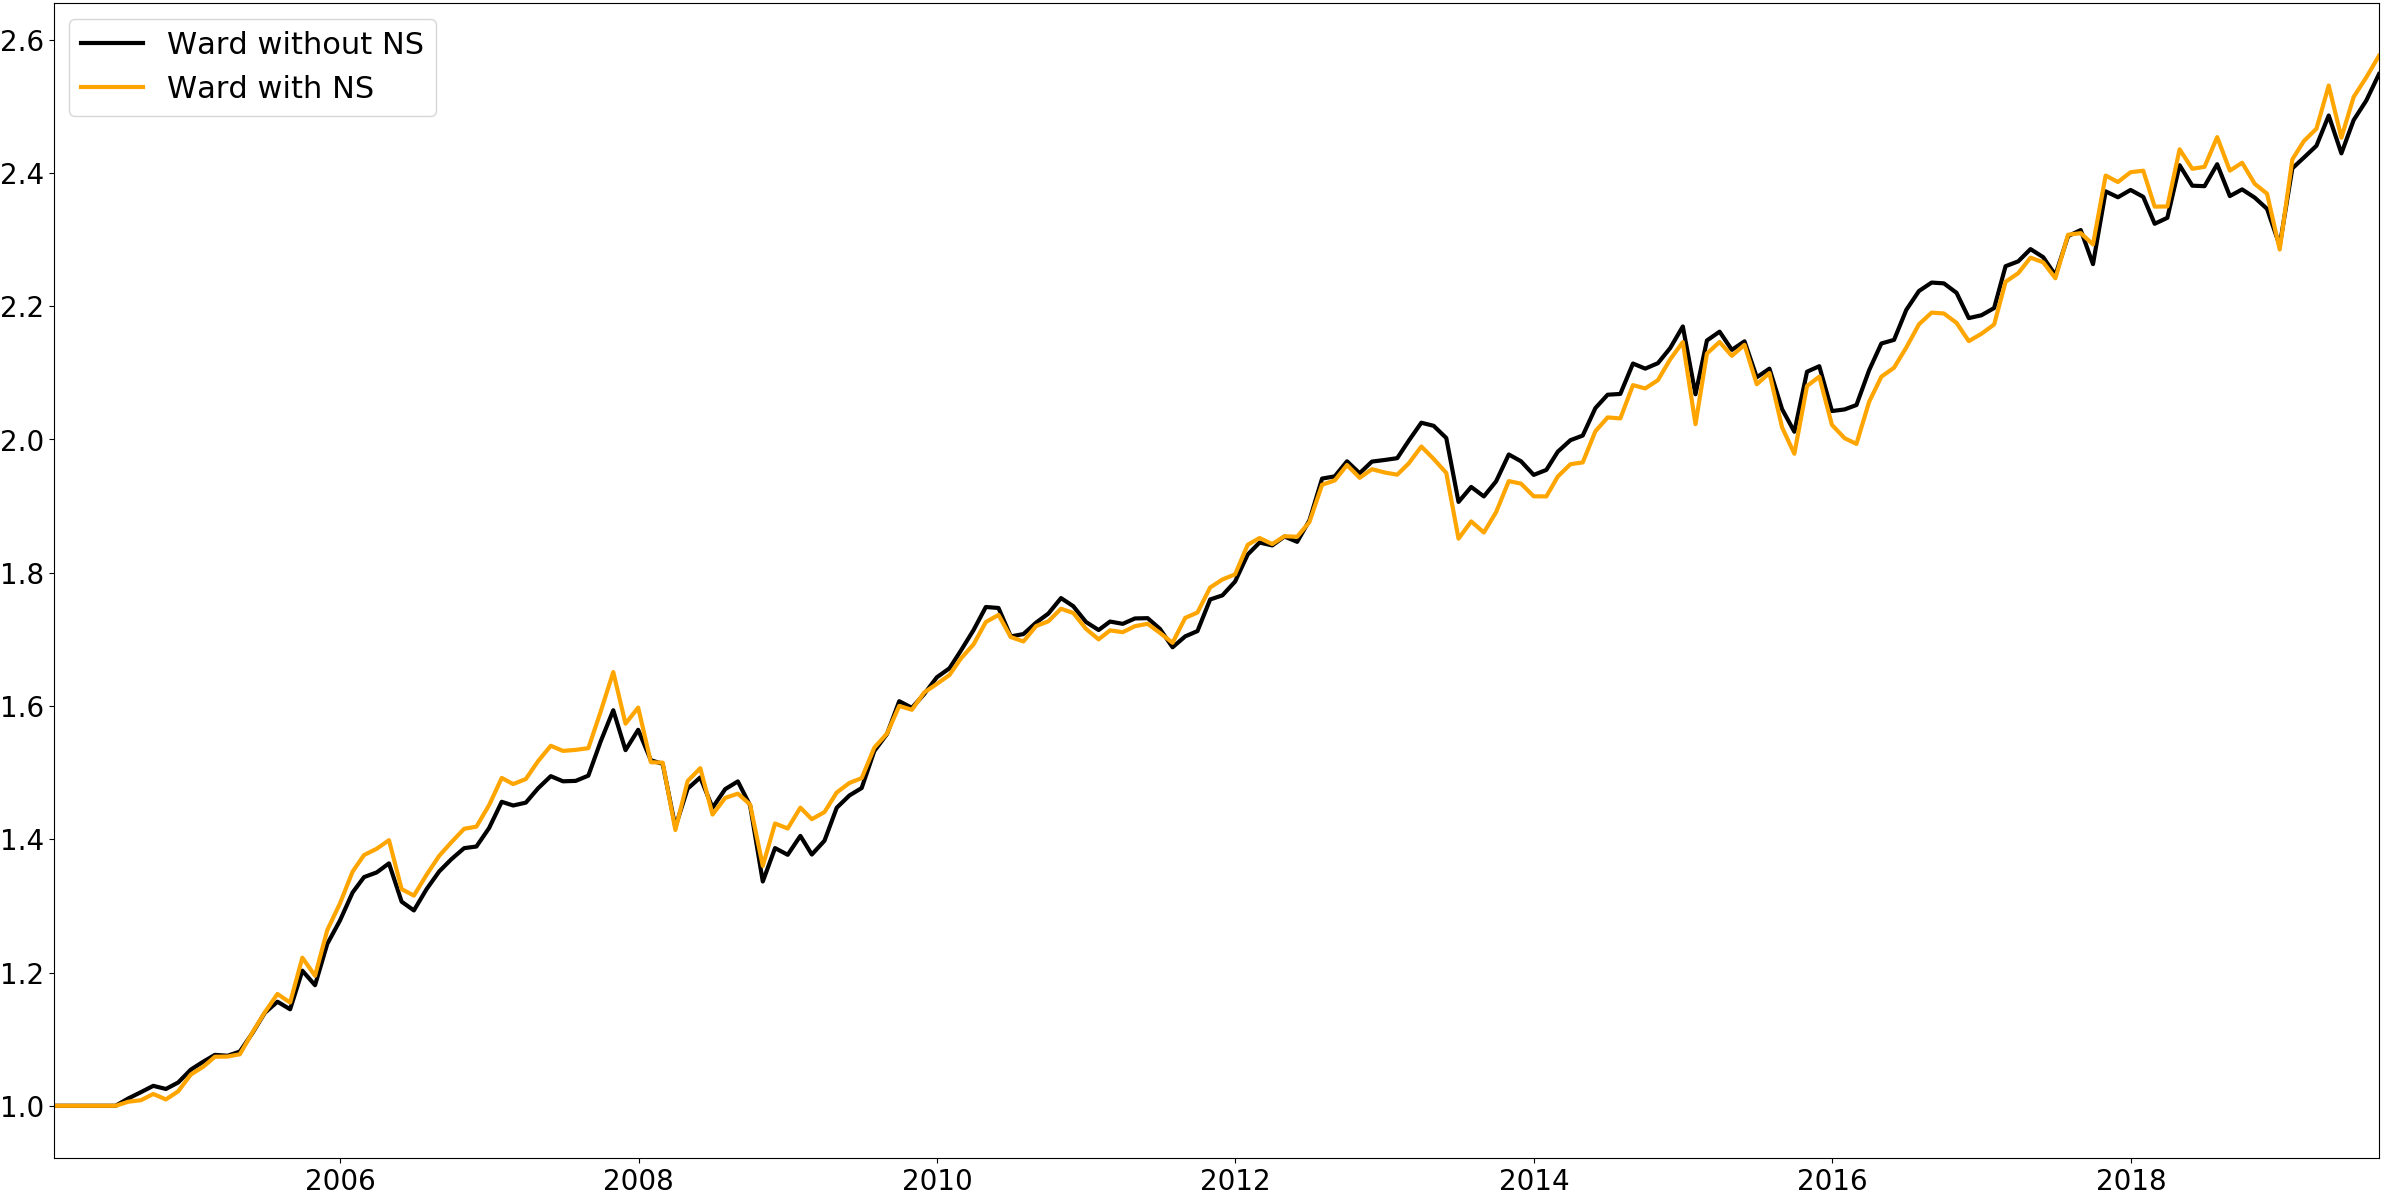
\includegraphics[width=\linewidth]{Plots_and_Tables/perf_noTC_ward_comp_F_2_B_0_LB_12_5_!!}
\caption{Comparison \texttt{ward} clustering approach with and without News Sentiment starting in July 2004.} \label{fig:tc_noNS_perf}
\end{subfigure}%\hspace*{\fill}


\medskip
\begin{subfigure}{0.8\textwidth}%{0.48\textwidth}
\centering
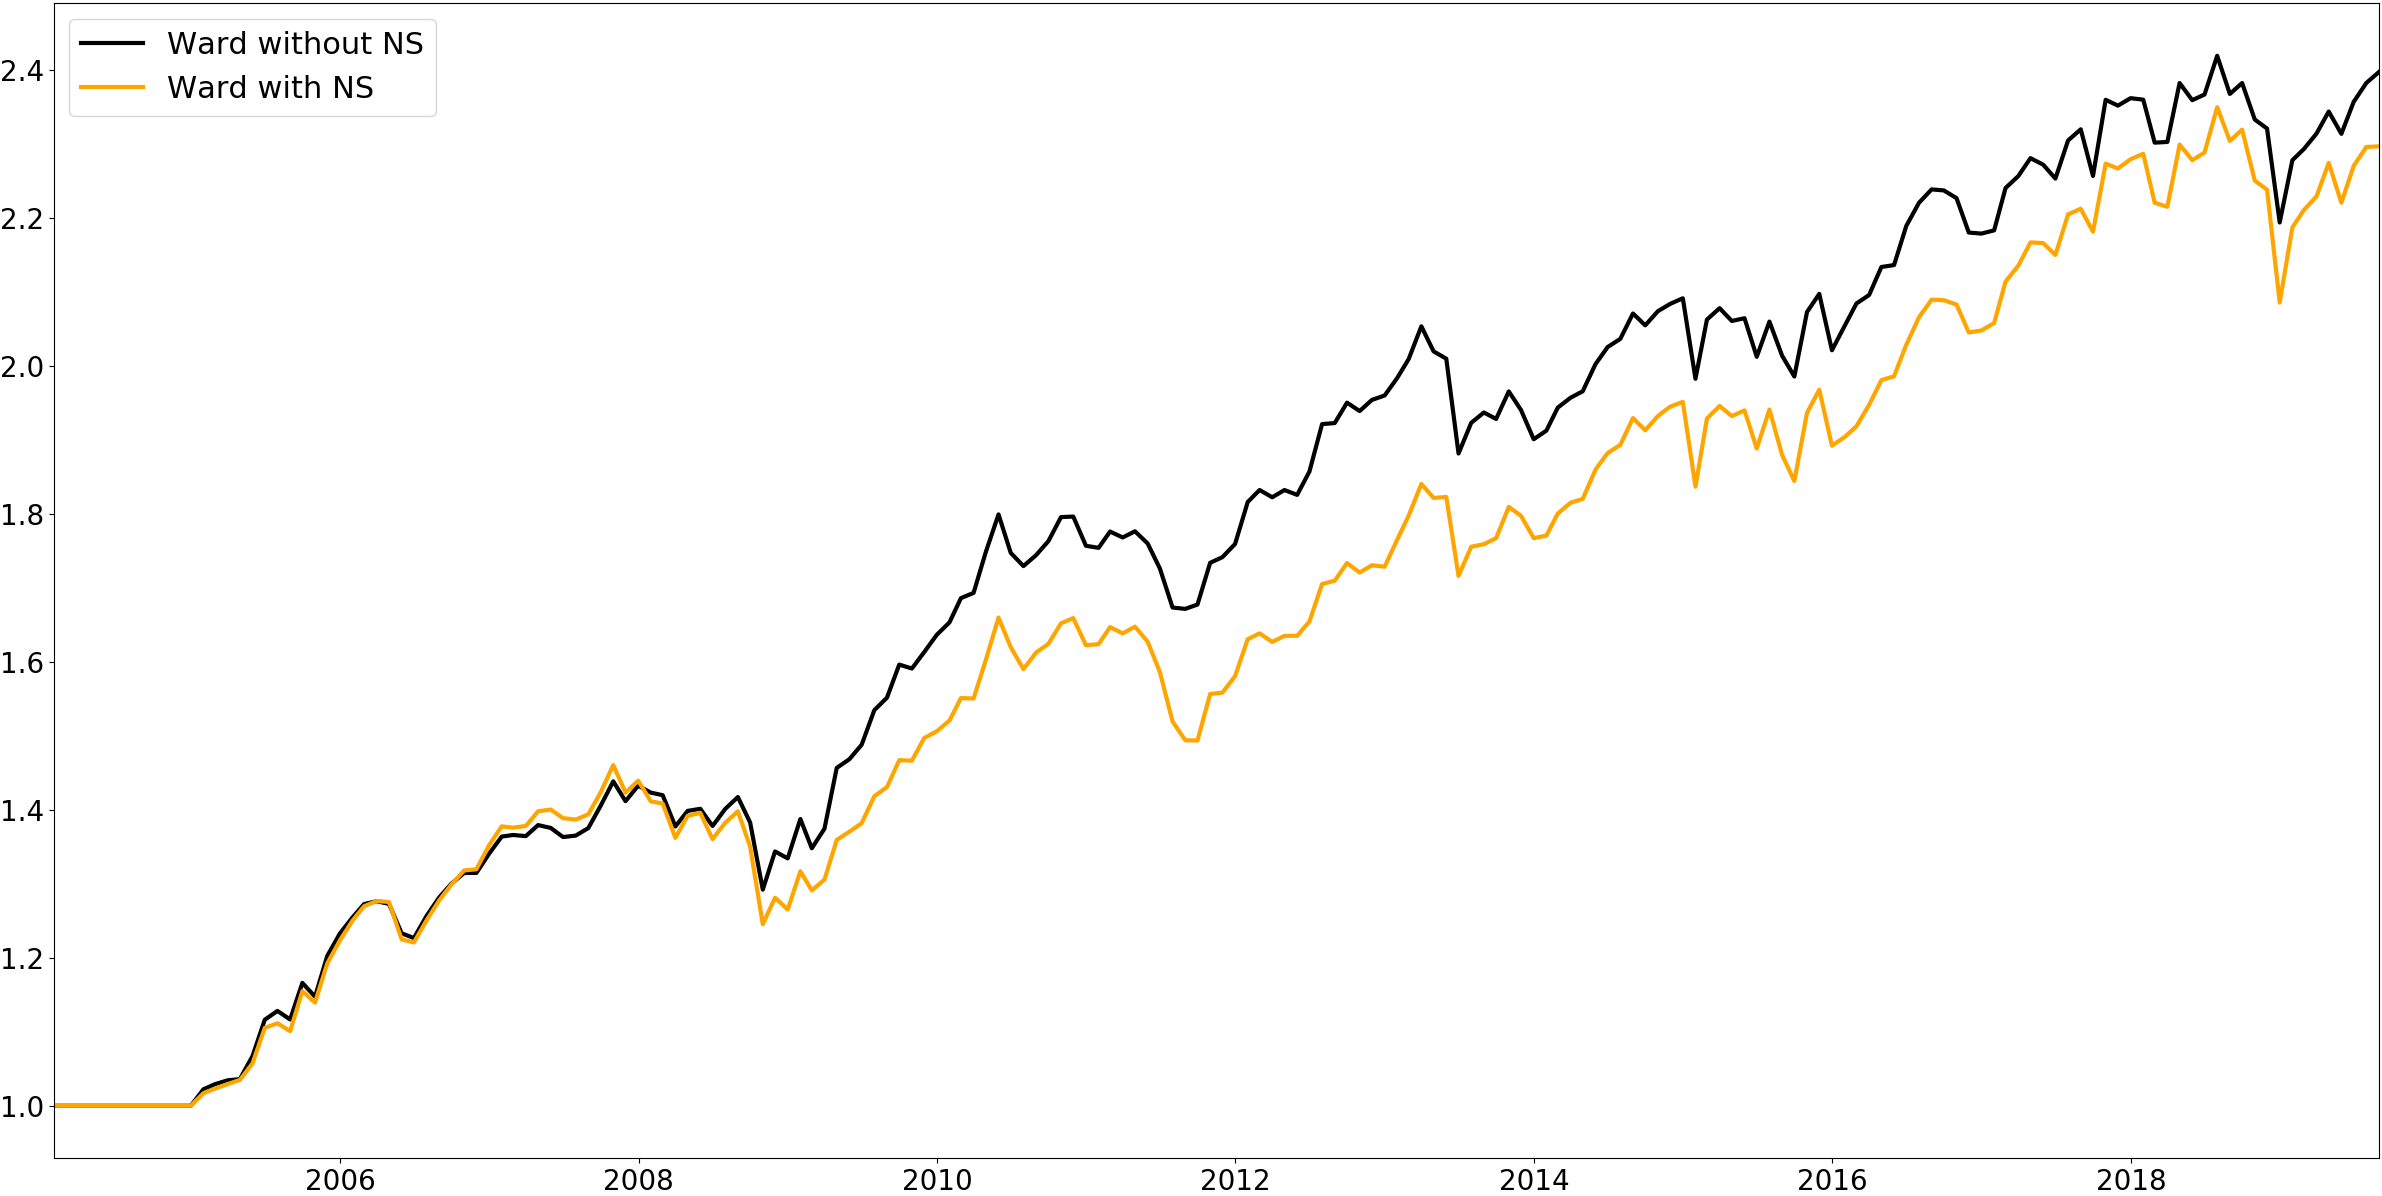
\includegraphics[width=\linewidth]{Plots_and_Tables/perf_noTC_ward_comp_F_2_B_0_LB_12_11_!!}
\caption{Comparison \texttt{ward} clustering approach with and without News Sentiment starting in January 2005.} \label{fig:comp_noNS_perf}
\end{subfigure}%\hspace*{\fill}


\caption{Performance of different strategies without News Sentiment enhancement.} \label{fig:noNS_perf}
\end{figure}
\newpage
\newpage
\section{Conclusion}

The idea of regime switching is not new. Indeed, it has become popular through the work of \citet{ang2004regimes} and \citet{hamilton1989new}. Nevertheless, the underlying model is hard to estimate and has limited practical applicability. With the emergence of machine learning techniques and News Sentiment analysis, alternative models where data is allowed to speak for itself become more realistic.

Our work derives from the research done by \citet{enhPortOpti} but we follow a model free approach in order to circumvent the limitations of mean variance optimization. As such, we rely on the HCBAA approach which was first introduced by \citet{de2016building} and later refined by \citet{raffinot2017hierarchical}. Our data set includes a variety of asset classes and the selection and hedging of the asset classes assumes an investor based in Switzerland. 

In a first step we construct four portfolios, each based on a different hierarchical clustering method and we report their performance against two benchmarks, an equally weighted portfolio and an inverse volatility weighted portfolio. Overall, all four portfolios outperform the benchmarks in terms of geometric Sharpe Ratio and monthly geometric average total return. However, the portfolio performances vary when the starting month of the backtest is changed but the portfolio relaying on the "ward" methodology seems to be the best performer overall.

In a second step, we introduce macro-economical News Sentiment as a way to adjust our exposure to risky assets. The riskiness of the assets is solely based on their beta. However, we are unable to draw a conclusion on the effectiveness of the News Sentiment enhancement as the enhanced portfolio can under perform depending on the starting month of the backtest. This could be due to the nature of our implementation as we only use one global macro News Sentiment variable. Thus, as future research it would be desirable to obtain News Sentiment time series for each individual asset and adjust exposure accordingly. Furthermore, it would be of interest to see what would happen if the trading window is decreased. However, this was outside of our scope of interest as we focused on Strategical Asset Allocation and not Tactical Asset Allocation.



\newpage
\printbibliography

%%%%%%%%%%%%%%%%%%%%%%%%%%%%%%%%

\end{document}
